\iffalse
\documentclass[journal,12pt,twocolumn]{IEEEtran}
\usepackage{amsmath,amssymb,amsfonts,amsthm}
\usepackage{txfonts}
\usepackage{tkz-euclide}
\usepackage{listings}
\usepackage{gvv}
\usepackage[latin1]{inputenc}
\usepackage{adjustbox}
\usepackage{array}
\usepackage{tabularx}
\usepackage{pgf}
\usepackage{lmodern}
\usepackage{circuitikz}
\usepackage{tikz}
\usepackage{graphicx}
\usepackage[english]{babel}

\begin{document}
\bibliographystyle{IEEEtran}

\vspace{3cm}

\title{}
\author{EE23BTECH11047 - Deepakreddy P
}
\maketitle
\newpage
\bigskip

\noindent \textbf{32} \quad An analog signal is sampled at 100 MHz to generate 1024 samples. Only
these samples are used to evaluate 1024-point FFT. The separation between
adjacent frequency points ($\Delta$F) in FFT is \rule{1cm}{0.5mm} kHz.\\
\hfill (GATE BM 2021)\\
\solution
\fi

\begin{center}
    \begin{table}[ht]
        \setlength{\arrayrulewidth}{0.3mm}
\setlength{\tabcolsep}{12pt}
\renewcommand{\arraystretch}{1.3}


\begin{center}
\caption{Input Parameters}
\begin{tabular}{ |p{1.7cm}|p{1.7cm}|p{1.7cm}|  }

\hline
 {Symbol}&{Description} & {value}\\
\hline
$f_s$ & Sampling frequency & 100 MHz\\
\hline
$N$ & No of samples  & 1024\\
\hline

\end{tabular}
\end{center}

    \end{table}
\end{center}

\begin{align}
    \Delta F &= \frac{f_s}{N}\\
    \Delta F &= \frac{100}{1024} MHz\\
    \Delta F &= \frac{10^5}{1024} kHz\\
    \Delta F &= 97.66kHz
\end{align}


\begin{figure}[ht]
   \centering
   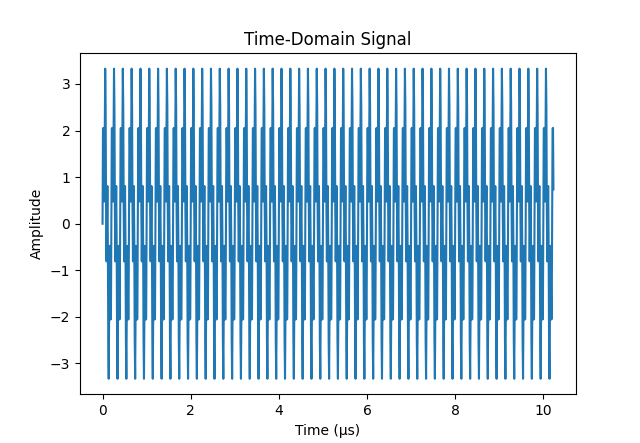
\includegraphics[scale=0.49]{2021/BM/32/figs/fig1.png}
   \caption{Time Domain Signal}
\end{figure}

\begin{figure}[ht]
   \centering
   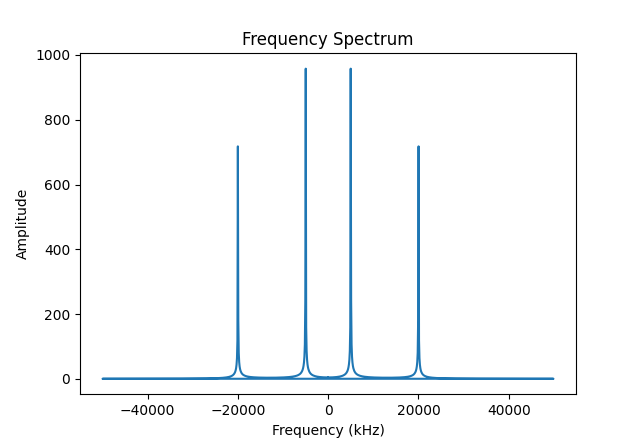
\includegraphics[scale=0.5]{2021/BM/32/figs/fig2.png}
   \caption{Frequency Spectrum}
\end{figure}






%\end{document}

